\section{PCB Layout}
Now, we can start the layout process, in this order :

\begin{itemize}[noitemsep]
    \item   Place the remaining components on the board
    \item   Route sensible tracks.
    \item   Route the remaining tracks
\end{itemize}

\subsection{Component placement}
Our board is quite big for the components we needed to place. Thus, there is
some empty space, which is not a bad thing.

This also mean that the placement of passive elements (which are, for most in
the package size 0603) was easier, since circuits are physically distants from
others.

For each circuit, we always start with the decoupling capacitors, that need to
be carefully placed near each power pins of the circuits. Then, we place the
remaining passives that can be placed farther from the chip, for example pull
up resistors.

This whole process was iterated two times. On the first pass, we globally place
the components, within 2 or 3 mm of their final position. Once the whole board
was done, we've got a first idea of what the board was going to look, but there
were a lot of smaller optimization that could be done. That's the goal of the
second pass, we replace every component to a place that can be easier to route,
aligned with the grid.

\subsection{Pin swapping}\label{sec:pin_swap}
For the next step, we configured the "pin swapping" function on the schematic,
to enable some pins to be swapped. This is possible due to the architecture of
most recent microcontrollers, where all of the functions goes trough a pin
matrix to assign to a pin, regardless of the peripheral. This gave us freedom
on the crossing that can be deleted with it \footnote{ This pin swapping method
    caused us some problems, because of an undocumented limitations : A peripheral
    can't use, at the same time multiples pins from different ports. This required
    us to re-route some part of the PCB. }.

We created four groups of pins :
\begin{itemize}[noitemsep]
    \item   A digital group on the port where the function is pinned to the port 0.
    \item   Another digital group, for the port 1.
    \item   An analog input group.
    \item   A global group, for independant pins that can be used on any port.
\end{itemize}

Then, the ECAD tool enable us to automatically perform pin swapping to globally
optimize the pins. Then, when routing, we can perform some precision pin swaps
if it can make the layout even easier.

\subsection{Layout}
When routing the connections, we've always got in mind the signal integrity
issues than may come from layout issues. Thus, we make sure that any fast
signal \footnote{ In fast, near every signal on the board can be qualified as
    fast, due to their rising and falling edges. Nonetheless, for signals that
    enable or disable functions once in the flight, we assumed that their behavior
    when switching aren't going to perturb the overall execution. } is routed on
top layers, or, by default with a ground plane near it to act as a return path
for the currents and a reference.

For every signals, if they need to "cross" a signal, on another layer, we
ensured the crossing to be at a 90 degrees to reduce the crosstalk between
them. In the same manner, we ensured that sensible tracks won't couple
inductively. This is done by separating them with enough space \footnote{A
    General rule of thumb is the 3W rule. Track center to the next center, there
    shall be 3 times the width. }.

For every track, we needed to route with a correct width, to ensure the current
carrying capacity will be large enough. Thus, for power tracks such as the 5V
rail for the servo engines, or the engine starters, we respectively used 1.5mm
wide tracks. For the 3.3V rail, that power up all of the logic, the current is
smaller, a 1mm wide track is more than enough.

To be added, in areas where a lot of pads share a single net, we used planes
rather than tracks to connect them. It make the layout easier to manufacture,
because we then get a single copper area rather than a dense track network.
This also increase the current carrying capacity on this point, for a zero
cost.

To place tracks in a cleaner way, we divide by two the grid, enabling us the
ability to pass exactly in the middle of two pins, to arrive right to the
center of a pad.

All of this work is shown on the images below, where we can see each layer,
individually, with the standard Altium color code.

\begin{figure}[!hbt]
    \centering
    \begin{minipage}[c]{\SmallSchematicWidth}
        \centering
        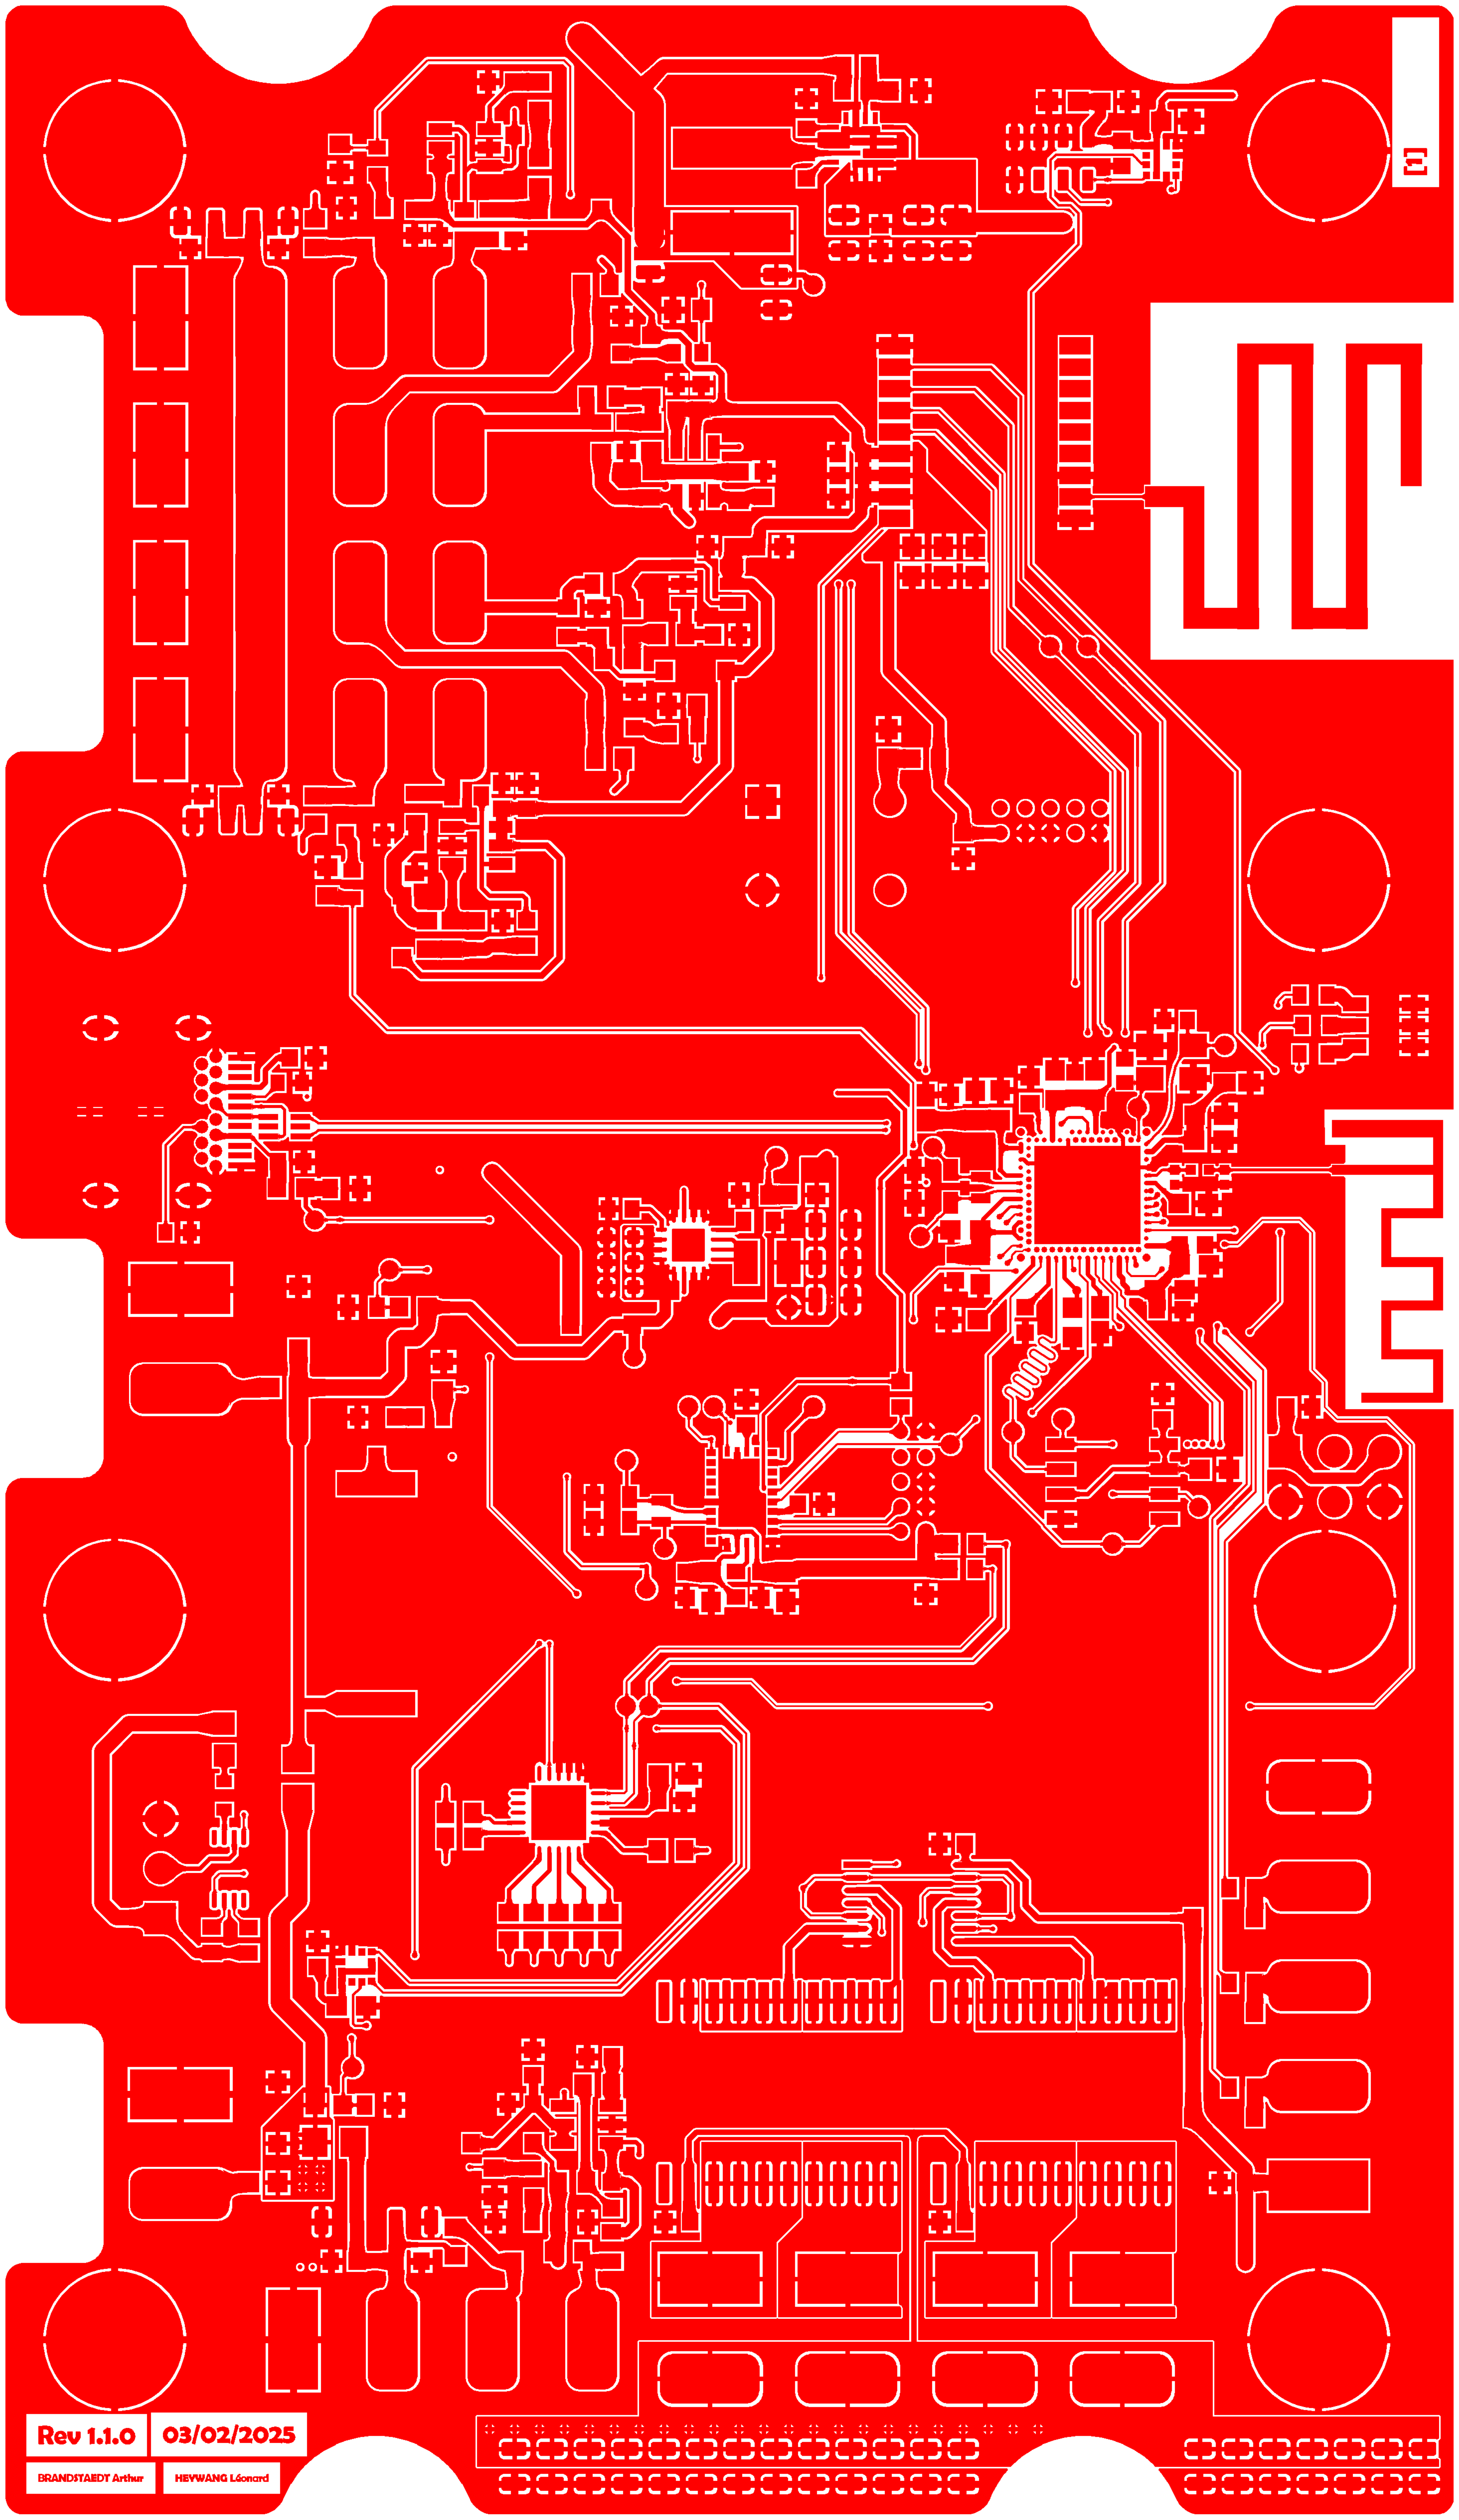
\includegraphics[width=\textwidth]{\Images/PCB/top.eps}
        \caption*{Copper layer (L1)}
    \end{minipage}%
    \hfill%
    \begin{minipage}[c]{\SmallSchematicWidth}
        \centering
        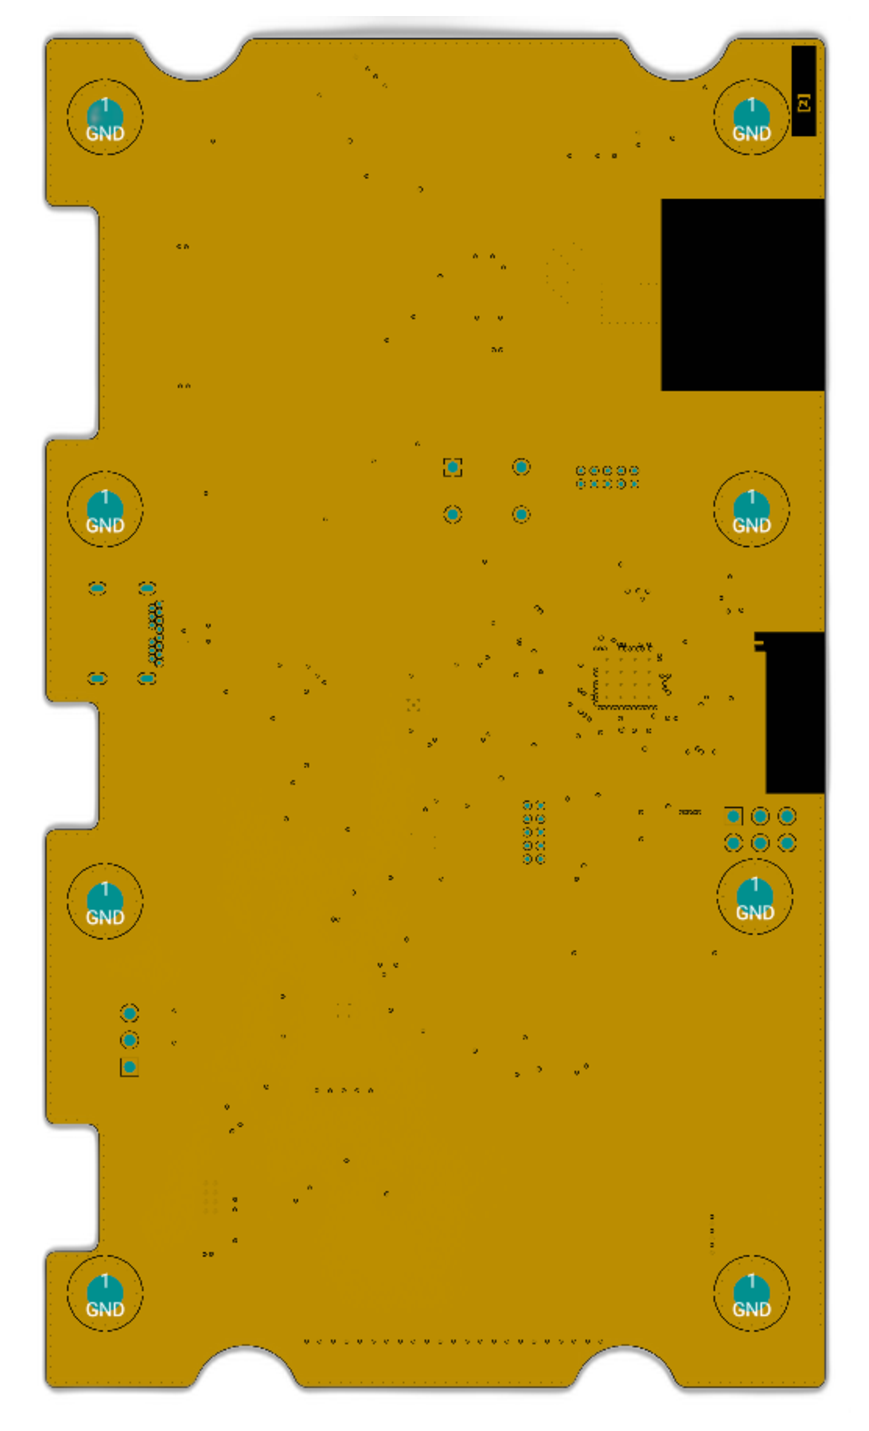
\includegraphics[width=\textwidth]{\Images/PCB/int1.eps}
        \caption*{Copper layer (L2)}
    \end{minipage}%
    \hfill%
    \begin{minipage}[c]{\SmallSchematicWidth}
        \centering
        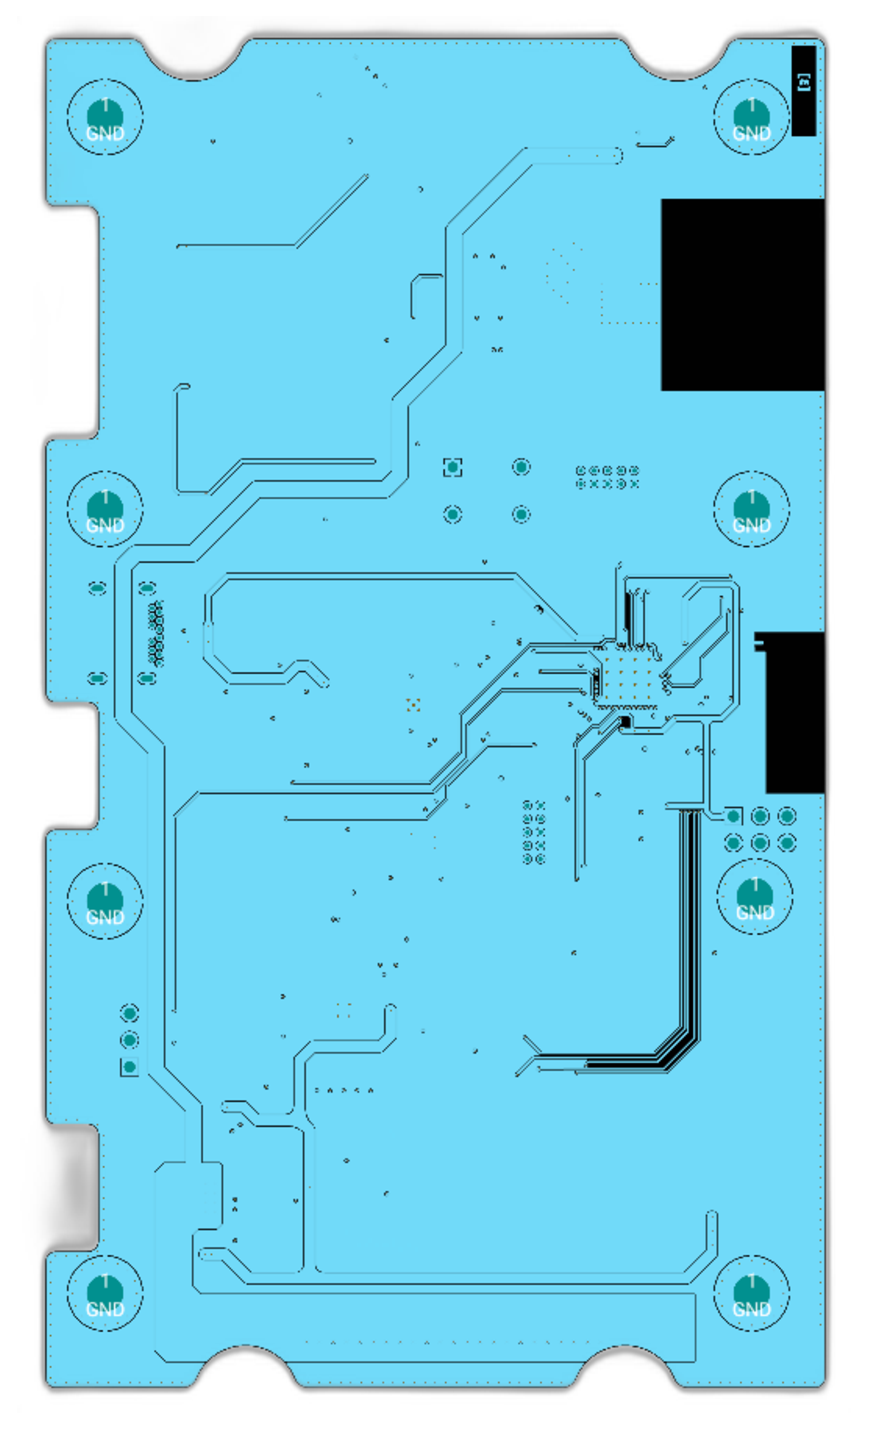
\includegraphics[width=\textwidth]{\Images/PCB/int2.eps}
        \caption*{Copper layer (L3)}
    \end{minipage}%
    \hfill%
    \begin{minipage}[c]{\SmallSchematicWidth}
        \centering
        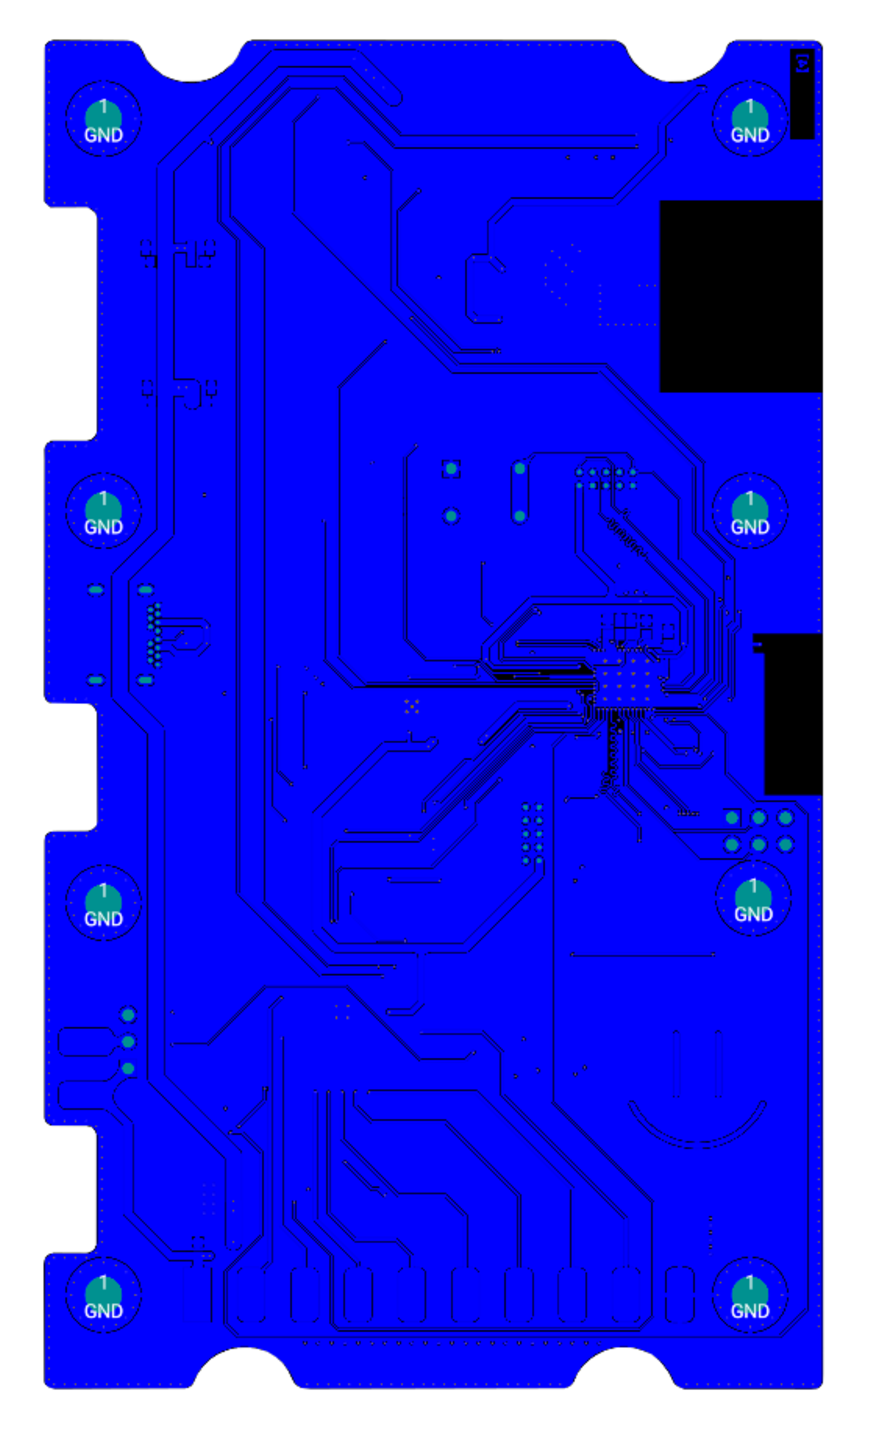
\includegraphics[width=\textwidth]{\Images/PCB/bot.eps}
        \caption*{Copper layer (L4)}
    \end{minipage}
    \label{img:layout}
    \caption{Copper layers on the PCB}
\end{figure}
\FloatBarrier

As explained before, we can cleary see that the first (L1) and last (L4) layers
are the most filled with tracks. The second layer (L2) is effectively empty of
traces, to let the space for a whole ground plane, and, on the last layer there
is the mix of both.

Once the layout was finished, we did some more steps to make the PCB cleaner :

\begin{itemize}[noitemsep]
    \item   Adding space betweens tracks if it can be done.
    \item   Placing the silkscreen designators and logos on the PC\footnote{ We ensured
              that designators were placed in two precise directions : Facing bottom of the
              board, or facing right side. This ensure some consistency in the overall
              design. }
    \item   Adding silkscreen notes to identify important pads.
\end{itemize}

Naturally, we ran a DRC (Design rules check) to ensure the PCB respected
manufacturing rules.

To go a bit further, the whole assembly process is available in the annexes of
the report : \ref{sec:assembly} and \ref{sec:defaults}